\chapter{Testing}

\begin{chapterabstract}
    Unit testing, system testing, usability testing and gained insights.
\end{chapterabstract}

Testing is an integral part of the software development process. This chapter provides an overview of the tests conducted during the development of this solution, as well as an evaluation and discussion of the testing results.

Software testing is essential for detecting malfunctions that may negatively affect the application's users and create further issues for the operator of the software. Testing is also necessary to confirm that the solution complies with the set specifications and helps to validate the design choices made. \cite{Homes2012}

There are various types of software tests, which can be categorized in many different ways, such as automated versus manual, functional versus non-functional, black-box versus white-box, by their coverage (unit versus whole system) or by their scope (performance versus compatibility). The choice of tests is always context-dependent and needs to be aligned with the project goals and limitations. \cite{Krysik2023}

Testing 3D applications presents unique challenges that differentiate it from testing standard web applications, with main differences in user interactions. The developed solution enables users to move within a 3D space and interact with spatial objects. All interactions therefore occur in a 3D environment projected onto a 2D viewport, significantly expanding the range of possible interactions compared to traditional 2D applications. The potential interactions also vary depending on the product being configured in the application, as the solution aims to be product-agnostic, as well as further complicating matters with the configurator's open navigation mechanism.

Unlike 2D applications where layout and style are the focus, 3D applications require tests to confirm that objects appear correctly from various angles and under different conditions. This aspect is challenging, as it is less straightforward than verifying the DOM of a standard website, since in this scenario, the 3D preview is represented by a canvas element without an easy method for breakdown. In addition, loading 3D content is time and computationally consuming, which makes testing resource intensive. These complexities limit the applicability of certain types of tests, such as automated browser testing, which typically does not accommodate the nuances of working with 3D content.

Given these constraints and the goals of the solution, three distinct kinds of tests were performed during the development lifecycle of the application: unit tests, system tests, and usability tests. The tests performed are described in the following sections.


\section{Unit Testing}

Unit testing involves testing the smallest parts of the software, which are typically individual functions. The testing is performed in isolation from the rest of the system, with dependencies being mocked or stubbed to ensure that the tests are independent. These tests provide immediate feedback on the functionality of the written code and help detect bugs or regressions when the code undergoes changes during development. Since the resulting application is composed of these integrated parts, validating these parts helps with the validation of the whole software. \cite{Khorikov2020}

\begin{listing}[h!]
\begin{minted}{typescript}
describe("CatalogActions.getCatalog", () => {
  test(
    "returns the existing catalog " 
    + "if already present in the store",
    async () => {
      const existingCatalog = generateMock(CatalogSchema);
      storeMock.catalog = existingCatalog;

      const catalog = await CatalogActions.getCatalog(
        "http://example.com/catalog",
        storeMock);

      expect(fetchCatalog).not.toHaveBeenCalled();
      expect(catalog).toBe(existingCatalog);
    }
  );
});
\end{minted}
\caption{Example unit test used to validate store action within the solution}
\label{listing:unit-test}
\end{listing}

Due to the technologies chosen and the nature of the developed solution, the majority of the codebase is made up of code visualizing the products, written in markup language. This type of code is unsuitable for unit testing as it does not encompass any logic. However, parts of the solution that involve manipulation of data schemas in stores require logic, and therefore, these parts of the solution were subjected to unit testing.

The tests are stored in the \texttt{src/\_\_tests\_\_} directory. For the purpose of unit testing, the Jest framework\footnote{\url{https://jestjs.io}} was used, which enables a streamlined definition and execution of the tests. These tests can be run by executing the command \mintinline{bash}{npm run test}. Although tests should be isolated, they still operate with some data; therefore, these data schemes need to be mocked. Because data schemas were defined using the Zod framework (see \autoref{section:data-schemas}), the zod-mock along with faker packages were used to quickly generate fake data from the schemes to be used in these tests, which closely resemble the values that will be used in real-world scenarios. An example of a defined unit test can be seen in \autoref{listing:unit-test}, which illustrates the generation of the mocked data, the calling of the tested function, and the verification of the results. Other unit tests are very similar to the illustrated one.

These tests validate the logic within the application and were run on commit to confirm the integrity of the changes made to the code during the development process.

\section{System Testing}

System testing verifies that all integrated components and subsystems of the solution work as expected. This type of testing verifies that the application behaves as expected from the perspective of the user and that it meets the specified requirements. \cite{Stephens2023}

Due to the specifics of this solution outlined at the beginning of this chapter, this testing was not automated and was performed periodically manually during implementation. When defects were found, they were immediately addressed. Therefore, the evaluation of the fulfillment of the requirements, which should result from this testing, was done periodically and is described at the end of the implementation chapter (see \autoref{section:requirmenets-evaulation}).

To streamline this manual testing process, automatic deployment of the development environment was enabled using the GitLab CI/CD pipeline, which was triggered after each change to the codebase. To assess various different functionalities of the application, several different products, such as shelves or PC configurations, were created to enable the system testing process. 

To ensure the compatibility and responsiveness of the application across different browsers and operating systems, the LambdaTest platform\footnote{\url{https://www.lambdatest.com/}} was utilized. This platform enables the testing of web applications on thousands of combinations of the major browsers and operating systems. \cite{LambdaTest}

Therefore, the application was tested on a relevant sample of browsers. The solution is designed to be compatible with all major browsers (Chrome, Firefox, Safari, Opera, Edge) with versions released from the year 2022 onward.


\section{Usability Testing}

Usability testing evaluates the functionality of the entire web application. In contrast with the system testing described in the previous section, usability tests use real users. They are carried out by a facilitator, along with a selected sample of users, who perform tasks representative of actual usage situations. The facilitator observes the users as they complete the tasks, noting their interactions with the system and their reactions. This allows to measure effectiveness, efficiency, and satisfaction of using the software. Usability testing is important, as it validates the proposed design from a fresh point of view, as the perception of the developed solution is different between the developer, who already knows every detail of the application, and the user, who has to learn how to work with the application.~\cite{Barnum2021}

Various categories of usability tests can be performed to assess different aspects of usability. Quantitative testing focuses on gathering numerical data about user experience, while qualitative testing collects observations and subjective feedback. In moderated testing, the user is led by the facilitator, compared to unmoderated testing, where the user is acting independently. Testing can be done remotely or in person, depending on available resources. \cite{Moran2019}

\subsection{Test Plan}

Before the actual testing process takes place, it is necessary to establish what is tested, in what manner, who are the test participants, and how is the testing conducted and evaluated. The following section discusses these aspects of the solution's usability testing.

In this thesis, usability testing is performed only on the configurator application. As discussed in the introduction of this thesis, the enjoyment of the configuration process itself directly influences the perceived value of the configured product~\cite{Franke2010}, therefore, it is imperative to ensure that the customer-centric configurator application is highly efficient and provides a great user experience in order to maximize the satisfaction of customers using the tool to configure their products.

Although usability testing could also be extended to the administrator part of the toolkit, it is important to note that the administrator application will be used only by administrators, which are only a few compared to the users of the configurator application. Administrators are also expected to have better technical knowledge than ordinary customers. The administrator part of the toolkit is conceived to be used infrequently, typically during the initial setup of the tool or for occasional updates of the product catalog. Given these factors, the configurator part of the toolkit must comply with usability standards higher than those of the administrator part; therefore, the available testing resources are better allocated entirely to the configurator application.

Usability testing was performed in person and in locations that are natural to the participants, either at their workplaces or at their homes. Since the solution requires no installation, the test participant's personal device was used to simulate real-world conditions and keep the participants comfortable.

The comfort and familiarity of the test participant are important during the testing process, as anxious users can skew the results by not reacting the same way as they would naturally when using the tool outside of a testing context.~\cite{Nielsen1994}

Based on analysis of usability testing, research has revealed that, on average, five test participants are enough to reveal around 85\% of usability flaws, with additional participants providing diminishing returns in terms of unique feedback. \cite{Nielsen2000} For this reason, the usability test was performed with five different users to efficiently gather as much comprehensive information as possible without overly intensive testing.  

During testing, standard approaches were followed. These include recording the sessions to enable more objective processing afterward. The testing process was clearly explained, making it known to the participant that the solution is being tested, not the user, and therefore they are free to express themselves and will not be judged. In addition, the facilitator aimed to conduct the test in a way that does not lead or influence the test participant by helping in any way or asking suggestive questions during the testing process.~\cite{Moran2019}

\subsubsection{Evaluation Methods}

Usability testing was performed using both qualitative and quantitative methods.

To gather important context before the testing process, participants were, along with their general profile, asked about the following information: 
\begin{enumerate}
    \item Does the participant have any previous experience with online product configuration, has the participant ever used similar tool to preview or order a product?
    \item Does the participant have experience with 3D computer programs?
    \item When ordering custom products, does the participant prefer personal contact, such as phone or email communication, or would they rather use an online configurator?
\end{enumerate}
This information is relevant, as the 3D controls employed in the developed solution are common; therefore, previous experience could impact the results of the usability test. In addition, the sentiment regarding the preferred shopping process could also influence the perceived usability of the tool.

During the process, the actions of the participants were observed and the think-aloud method was used.

With the think-aloud protocol, participants are encouraged to reveal their thoughts during the process and to think out loud when using the application. This means that along with the actions taken, the information about why they have taken it is also immediately captured. \cite{Moran2019}

After the test, a qualitative evaluation was done by conducting an interview with a general discussion about the solution, including the following questions:
\begin{enumerate}
    \item What difficulties did the participant encounter when using the tool? Was there anything particularly frustrating?
    \item What three improvements or features would the participant like to see?
    \item Did any part of the tool feel unnecessary or redundant?
    \item Is the product representation clear enough to understand what was configured?
    \item Would the participant use this tool in a real scenario to inquire configured products?
    \item What was the initial feeling about the tool?
\end{enumerate}

For quantitative evaluation, the System Usabilty Scale (SUS) questionnaire was used.

The SUS is an industry standard for quickly evaluating the usability of a system. It consists of 10 questions, each with a numerical response on a scale from one to five, one representing \textquote{strongly disagree} and five being \textquote{strongy agree}. The questions are presented in \autoref{table:sus}. \cite{Sus}

\begin{table}[htb]
\centering
\begin{tabular}{r>{\raggedright\arraybackslash}p{11.5cm}}
\toprule
1. & I think that I would like to use this system frequently \\
2. & I found the system unnecessarily complex \\
3. & I thought the system was easy to use \\
4. & I think that I would need the support of a technical person to be able to use this system \\
5. & I found the various functions in this system were well integrated \\
6. & I thought there was too much inconsistency in this system \\
7. & I would imagine that most people would learn to use this system very quickly \\
8. & I found the system very cumbersome to use \\
9. & I felt very confident using the system \\
10. &  I needed to learn a lot of things before I could get going with this system \\
\bottomrule
\end{tabular}
\captionsource{SUS questionnaire}{\cite{Sus}}
\label{table:sus}
\end{table}

A score is then calculated from the SUS in as follows:
\begin{itemize}[label=\rectanglebullet]
    \item The response values for odd-numbered questions are subtracted by one.
    \item The response values for even-numbered questions are subtracted from five.
\end{itemize}
The adjusted responses are then added together and multiplied by 2,5, giving a score between 0 and 100. This is calculated for each participant. To get a single value that rates the entire system, the average of these scores is taken. \cite{Sauro2011}

Research of 500 usability studies has shown that the average SUS score is 68. Therefore, a score above 68 suggests that the solution is better than the average system in terms of usability. However, it should be noted that this is a comparison with different types of systems, not necessarily with the same functionality. The 90th percentile is an SUS score of about 80,3. \cite{Sauro2011}

The time to complete the tasks was not measured, as product configuration is a creative process where speed does not necessarily mean better performance. 

\subsubsection{Scenario}

For usability testing purposes, a mock product, a modular kitchen countertop, was prepared for configuration within the tool, with configurable components such as drawers, sinks, cabinets, corners and smooth edges.

Consequently, a single test case was used that involved the configuration of the defined kitchen product. This test case was broken down into several subtasks that participants were instructed to complete using the configurator application.

In the scenario presented to the users, the background context involved them renovating their homes and being in need of a new remodeled kitchen. They found a company specialized in custom kitchen furniture, which utilized a website where they used the developed solution to handle inquiries. The user has visited the configurator, at which point the usability testing has started. The subtasks were as follows:
\begin{enumerate}
    \item Create a configuration of kitchen modules in \textquote{L} shape. The left part of the kitchen should include a drawer and sink, and the right part of the kitchen should contain two cabinets and another drawer.
    \item Add a smooth edges component to the edge modules.
    \item Set the color of the countertop of all the modules to \textquote{dark} and the wooden part of the modules to the color \textquote{cherry}. The color of the sink component should be set to \textquote{copper}, and the faucet to \textquote{gold} color.
    \item Review the created configuration and fill out and send an inquiry form with contact details.
\end{enumerate}

These product features and subtasks were selected to ensure that the majority of functionalities of the configurator application were tested by the users in a single, comprehensive test case, which represented the expected regular use. 

\subsection{Testing Process}

The following section describes the selection of participants for the usability test and provides a summary of the transcription from the testing process itself. 

\subsubsection{Participants}

As mentioned in the previous section, five participants were selected, which should be sufficient to uncover most usability issues. The participants were deliberately chosen to be heterogeneous, representing a range of different age groups, to ensure that the testing provided as much information as possible.

The participants, along with the contextual information gathered from them and the devices they used, are as follows:
\begin{enumerate}[label=\textbf{Participant \Alph*:}, leftmargin=*, itemindent=6.2em]
    \item 18 years old, male
        \begin{itemize}[noitemsep, label=\trianglebullet]
            \item \textbf{Experience:} Previous experience with 2D car configurator, also relevant experience with 3D modeling and extensive 3D gaming.
            \item \textbf{Device:} Desktop PC with Windows.
        \end{itemize}
        \vspace{4pt}
    \item 22 years old, female
        \begin{itemize}[noitemsep, label=\trianglebullet]
            \item \textbf{Experience:} Previous experience with 3D furniture configurator, also relevant experience with casual 3D gaming.
            \item \textbf{Device:} Mobile device with iOS.
        \end{itemize}
        \vspace{4pt}
    \item 46 years old, female
        \begin{itemize}[noitemsep, label=\trianglebullet]
            \item \textbf{Experience:} Previous experience with 3D furniture configurator, no other relevant experience.
            \item \textbf{Device:} Desktop PC with MacOS (with an Apple Magic Mouse).
        \end{itemize}
        \vspace{4pt}
    \item 52 years old, male
        \begin{itemize}[noitemsep, label=\trianglebullet]
            \item \textbf{Experience:} Previous experience with 2D car configurator, also relevant experience with 3D visualization software.
            \item \textbf{Device:} Laptop with MacOS (with a standard external mouse).
        \end{itemize}
        \vspace{4pt}
    \item 62 years old, female
        \begin{itemize}[noitemsep, label=\trianglebullet]
            \item \textbf{Experience:} No previous experience with configurators or other relevant experiences.
            \item \textbf{Device:} Laptop with Windows (with a standard external mouse).
        \end{itemize}
\end{enumerate}
All participants expressed a positive sentiment towards using a configurator tool instead of a direct inquiry process.

\subsubsection{Execution and Observations}

The testing process began by preparing the tested application on the device and ensuring that there would be no interruptions during the testing.

The usability testing process, its purpose, and principles were then explained to the participants along with the three stages that it consists of: pre-test questions, the test itself, and post-test questions.

Questions were asked to establish context about the participant's background, experience, and sentiment, as detailed in the previous sections. The responses can be found in the previous section along with other details about the participants.

The test of the application itself then began. The participants were reminded that it was the application being tested, not the user; therefore, they would not be judged and that any issues they may face are problems of the application's usability. Participants were also reminded that they would not be helped during the process but only observed, and were asked to think aloud and share their thoughts to help with this observation. The prepared scenario and the tasks they should complete were explained and presented to them on a sheet of paper for further easy reference. 

All participants immediately understood what to do and chose the initial component of the kitchen. The controls in the 3D space, along with the buttons for the addition of components, were also understood quickly by everyone. Therefore, the addition of the first components of the product was not problematic for anyone. 

However, as the configured product grew more complex, the addition of more components became an issue for everyone except Participant A. The problem was caused by an unclear scrolling pattern in the component addition menu. The menu pops up from the bottom of the screen, with horizontally laid tiles representing the mountable components. If there are more mountable components than would fit in this menu, horizontal scrolling is utilized. Due to the disappearance of the scroll bar and soft shading of the background, it was not clear to the participants that there could be more components accessible by scrolling horizontally. Although every participant has eventually figured it out, it has caused problems and frustrations, which, especially in the case of Participant C, lasted several minutes. Furthermore, Participant D has also suggested that a categorization of the available components on this panel would be beneficial for better orientation. 

Another observed pain point, which the majority of participants have also reported afterwards, was aggressive camera zooming. Whenever a component is selected, the camera tries to center the chosen component on screen. Almost all participants have reported that this movement is either too jarring and fast or that the zoom effect is too strong and that the 3D object should not be zoomed so much. 

\begin{wrapfigure}{r}{0.4\textwidth}
    \centering
    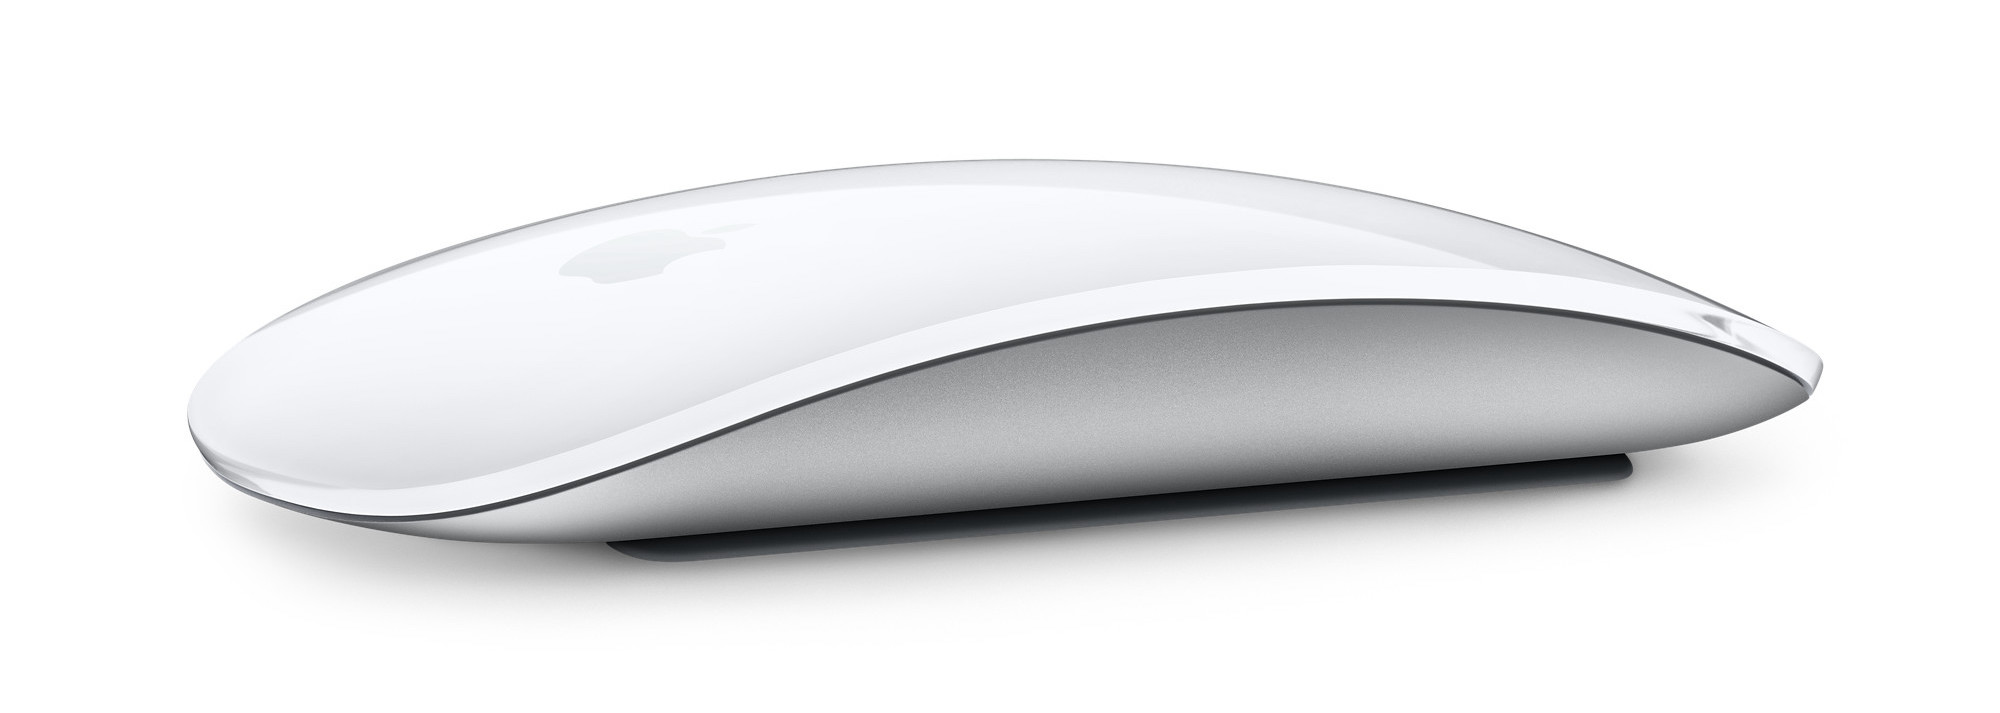
\includegraphics[width=0.35\textwidth]{images/image_magicmouse.jpg}
    \captionsource{Apple Magic Mouse}{Apple \cite{MagicMouse}}
    \label{fig:magic-mouse}
\end{wrapfigure}

Participant C, who used an Apple Magic Mouse with an unconventional button layout and gestures (see \autoref{fig:magic-mouse}), experienced particular difficulties. When trying to compensate for unwanted camera centering, the participant accidentally performed a gesture on the mouse to navigate away from the application, restarting the whole configuration.

In addition to the selectable components in the 3D view, as a supporting element, there is also a small button symbolizing the component that also allows users to select it. This button is positioned at the point where the component is mounted. This has caused small issues for Participant C and Participant E. The post-test discussion revealed that the problem was caused by two things: the base component does not have a mounting point, therefore, the application does not have a button for this component, and at the same time the position of the button on the mounting point caused confusion as it was unclear to which component the button belongs to. The participants implied that it would be more intuitive if the button was placed in the center of the component.

Participants C and E also encountered small issues with the remove component button, which uses a hold-to-confirm mechanism instead of the traditional confirmation pop-up. The unfamiliarity with this mechanism has led both participants to require three attempts to perform this action. 

Participant B expected that the review of components in the confirmation screen would be interactive, allowing for changes to the colors of the materials instead of merely reviewing them.

After overcoming these challenges, the participants quickly understood and completed the rest of the tasks without any further obvious problems. The participants were then asked to complete the SUS questionnaire on the second side of the instructions sheet, followed by an interview where the previously detailed questions were asked.

In the post-test interview, a common wish among all participants except Participant D was that the material color changes would apply to all components made of the same material, rather than having to adjust each one individually. Two participants also mentioned that the outline of the selected components was too wide and strong, obscuring the customized color. Participant B has also expressed the desire to have the ability to change the environments in which the product is visualized.

Participants deemed no part of the tool redundant, except Participant D, who considered the configuration review and confirmation screen unnecessary in the current form and suggested that a screenshot of the 3D preview of the configuration should also be included there.

When asked about their initial feeling, three participants expressed that they wanted a guide or tutorial to be presented on the initial screen, and two participants mentioned that having preset configurations with prearranged components would be beneficial.  

All of the participants regarded the 3D product representation to be clear and understandable and all expressed that they would use this application in a real scenario.

\subsection{Test Results}

The following section provides evaluation results and a summary of insights gained from the testing process, as detailed in the previous section.

The general sentiment regarding the usability of the tool was positive among all participants.

\begin{figure}[h!]
\centering
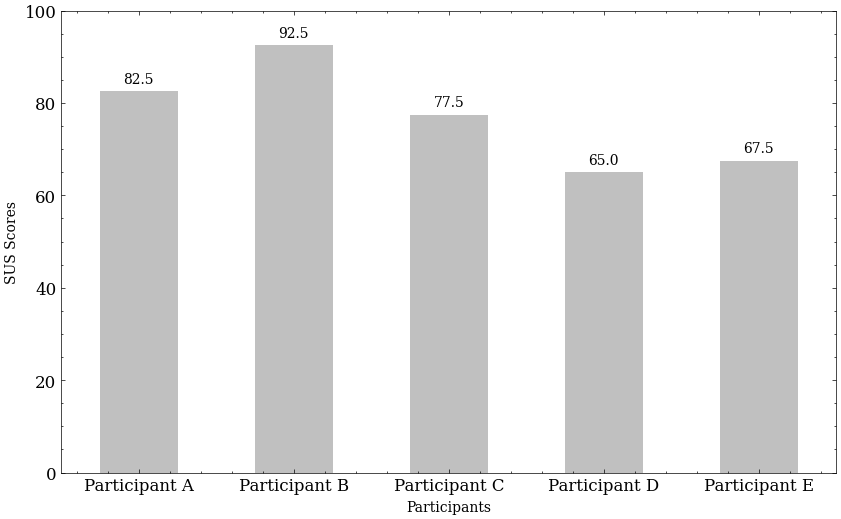
\includegraphics[width=0.95\textwidth]{images/graph_sus.png}
\caption{SUS scores by participant}
\label{fig:sus-scores}
\end{figure}


The average SUS score for all participants was 77 which is considered good and above average when compared to other systems. The lowest SUS score was 65, recorded for Participant D, and the highest was 92.5, recorded for Participant B. Scores for all participants are plotted on the chart shown in \autoref{fig:sus-scores}.

A trend appears to indicate that the tool is more suitable for younger users. However, given the small sample size, this does not provide enough evidence to draw statistically significant conclusions in this regard.

\subsubsection{Insights} \label{section:insights}

The following section summarizes the issues identified during usability testing along with potential improvements, describes how fixes could be implemented, and reports the current status of these implementations. In addition, the severity of each issue is estimated based on the difficulties observed during usability testing. The estimated severity was classified as high, medium, or low. The priority for implementing fixes was based on the estimated severity.

\begin{enumerate}[label=\textbf{I\arabic*:}, leftmargin=*]
    \item Unclear scrolling pattern in component addition menu
        \vspace{2pt}
        \\Horizontal scrolling in the menu is not apparent (see \autoref{fig:screenshot-add-before}), leading users to believe that there are fewer available components than there really are.
        \begin{itemize}[noitemsep, label=\trianglebullet]
            \item \textbf{Severity:} High
            \item \textbf{Proposed fix:} Arrow buttons should be added as an additional apparent scrolling mechanism
            \item \textbf{Implemented:} Yes, see \autoref{fig:screenshot-add-after}
        \end{itemize}
        \vspace{4pt}

        \begin{figure}[h]
        \centering
        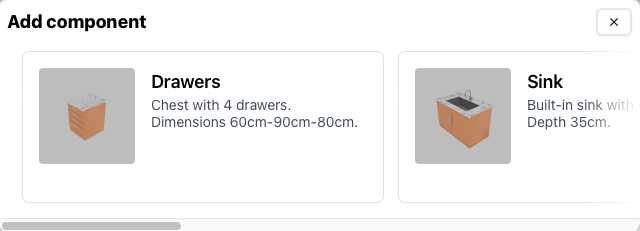
\includegraphics[width=0.7\linewidth]{images/screenshot_add-before.png}
        \caption{Component addition menu before implemented fix}
        \label{fig:screenshot-add-before}
        \end{figure}
        \begin{figure}[h]
        \centering
        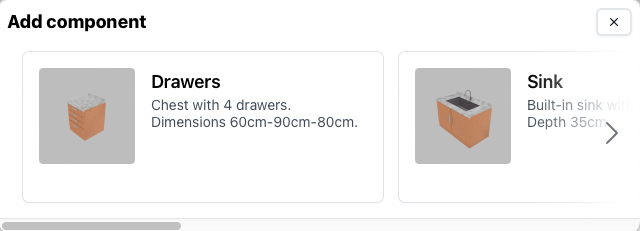
\includegraphics[width=0.7\linewidth]{images/screenshot_add-after.png}
        \caption{Component addition menu with implemented arrows for scrolling}
        \label{fig:screenshot-add-after}
        \end{figure}
    
    \item Jarring camera movement
        \vspace{2pt}
        \\The camera moves too abruptly and zooms in too much on component selection, causing discomfort and confusion among users.
        \begin{itemize}[noitemsep, label=\trianglebullet]
            \item \textbf{Severity:} High
            \item \textbf{Proposed fix:} The camera speed should be slowed down and limited to rotation only, avoiding zoom on component selection
            \item \textbf{Implemented:} Yes
        \end{itemize}
        \vspace{4pt}

    \item Incorrect position of the component selection button
        \vspace{2pt}
        \\The button supporting the selection of components is positioned at the point the component is mounted at, creating confusion about which component the button is associated with. The button is also missing on the base component.
        \begin{itemize}[noitemsep, label=\trianglebullet]
            \item \textbf{Severity:} Medium
            \item \textbf{Proposed fix:} The button representing the component should be centered within the 3D object and added also to the base component
            \item \textbf{Implemented:} Yes
        \end{itemize}
        \vspace{4pt}

    \item Excessive outline of the selected component
        \vspace{2pt}
        \\The outline of the selected component within the 3D preview can be too wide, obscuring the customized color of the component.
        \begin{itemize}[noitemsep, label=\trianglebullet]
            \item \textbf{Severity:} Medium
            \item \textbf{Proposed fix:} The width of the outline should be reduced or made transparent
            \item \textbf{Implemented:} Yes
        \end{itemize}
        \vspace{4pt}

    \item Lack of guidance
        \vspace{2pt}
        \\The tool does not provide users with any information about the controls.
        \begin{itemize}[noitemsep, label=\trianglebullet]
            \item \textbf{Severity:} Medium
            \item \textbf{Proposed fix:} A panel detailing the controls should be presented when first accessing the application and also accessible by a button at any time.
            \item \textbf{Implemented:} No
        \end{itemize}
        \vspace{4pt}

    \item Separated material changes
        \vspace{2pt}
        \\Changing the color of materials only affects a single component, even if there are other components with the same materials in the configuration. Therefore, updating the same material across all components requires individually adjusting each one.
        \begin{itemize}[noitemsep, label=\trianglebullet]
            \item \textbf{Severity:} Medium
            \item \textbf{Proposed fix:} The data scheme for material specifications should be revised to not be part of the components but to be shared between them, alternatively, changing the color of a material could automatically update all components with the same material identification
            \item \textbf{Implemented:} No
        \end{itemize}
        \vspace{4pt}

    \item Missing preset configurations
        \vspace{2pt}
        \\The configurator does not provide users with precreated configurations on which the user could build upon.
        \begin{itemize}[noitemsep, label=\trianglebullet]
            \item \textbf{Severity:} Medium
            \item \textbf{Proposed fix:} Administrator should be able to create and offer product configurations which the user can use to derive their own configuration
            \item \textbf{Implemented:} No
        \end{itemize}
        \vspace{4pt}

    \item Unintuitive hold-to-confirm mechanism
        \vspace{2pt}
        \\The confirmation action used on the delete button, which requires holding the button for a while, is unintuitive.
        \begin{itemize}[noitemsep, label=\trianglebullet]
            \item \textbf{Severity:} Low
            \item \textbf{Proposed fix:} The hold-to-confirm mechanism should be replaced with standard confirmation popup
            \item \textbf{Implemented:} No
        \end{itemize}
        \vspace{4pt}

    \item Confirmation screen does not allow changes
        \vspace{2pt}
        \\The confirmation screen only offers an overview, and to make changes to the colors of materials, it is necessary to return to the configurator screen. In addition, the confirmation screen could provide more information.
        \begin{itemize}[noitemsep, label=\trianglebullet]
            \item \textbf{Severity:} Low
            \item \textbf{Proposed fix:} Changing colors of materials should be enabled directly from the confirmation screen, and the screen should present a screenshot of the preview of the 3D configuration
            \item \textbf{Implemented:} No
        \end{itemize}
        \vspace{4pt}

    \item Lack of categorization in the component addition menu
        \vspace{2pt}
        \\Categorization of components in the addition menu would improve user orientation and ease of use.
        \begin{itemize}[noitemsep, label=\trianglebullet]
            \item \textbf{Severity:} Low
            \item \textbf{Proposed fix:} A new category data scheme should be implemented to encompass different component specifications, and the menu should group the components based on their respective categories
            \item \textbf{Implemented:} No
        \end{itemize}
        \vspace{4pt}

    \item Blank environment in the 3D preview
        \vspace{2pt}
        \\The 3D preview features a blank background set by the administrator, which can appear bland.
        \begin{itemize}[noitemsep, label=\trianglebullet]
            \item \textbf{Severity:} Low
            \item \textbf{Proposed fix:} Various 3D backgrounds should be introduced to allow visualization of the configured products in different environments
            \item \textbf{Implemented:} No
        \end{itemize}
        \vspace{4pt}
\end{enumerate}

Since only the most critical usability improvements were implemented, the remaining unimplemented usability enhancements could be the subject of further development of the tool and complement \autoref{section:improvements} on future improvements.
